\chapter{Methodology}

As mentioned in Chapter 1, the goal of this thesis was to develop an interface
for reinforcement learning research on StarCraft. The following sections
outline the process of design, implementation and testing of the platform.

\section{Specifications}

Obtaining a list of specifications for the platform was relatively challenging
for a few reasons: the design needed to provide a powerful environment while
maintaining a strong degree of expandability. With the sudden re-popularisation
of reinforcement learning the community has begun challenging previously
untouched problems, meaning that entirely new architectures might soon appear
and provide new constraints for existing platforms.

We identified the following minimal requirements:

\begin{itemize}
\item Ability to control StarCraft. This included (but was not limited to)
  starting, pausing, and ending games, killing and re-starting the program,
  selecting certain maps or campaigns.
\item Ability to collect and share game state information.
\item Ability to control the game from the player perspective
\item Ability to collect data from human players and replays available over the
  internet.
\item Ability to use hacks and / or some of the cheats the deactivate some of the
  features that make the general game particularly hard (say, fog of war). 
\end{itemize}

Additionally, because of the surge of deep reinforcement learning we placed the
ability to use one or some of the currently popular deep learning libraries on
top of the requirements list.

% Overall design

\section{Brood War Application Program Interface}

One of the main reasons this project became possible within the time constraint
was because of the existence of the Brood War Application Program Interface
(BWAPI). A closed-source game like StarCraft would normally be very hard to
control and to use as a learning platform, but thanks to a few extraordinary
developers it has been possible to build bots for game. BWAPI is a framework
written in C++ that provides a clean and modular interface to gain access to the
game data structures, allowing to collect game information and to control units
much in the same way a human player would.

BWAPI uses DLL injection to interact with the game, providing two interfaces to
the game: BWAPIModule and BWAPIClient. The first one allows to control of the
units through callbacks fired 
% (?????) 
by in-game events, so it's mostly suitable
for running agents that do not require to have complete control of the game (as
the game is configured centrally by the injected BWAPI.dll at startup). The
second interface allows to directly connect and interact with the server started
within BWAPI.dll, which gives the ability to arbitrarily control most of the
process state.
Even thought BWAPIClient lacked some documentation, we decided to use it to give
us the maximum amount of maneuverability later in the implementation phase.

\section{Pipeline Design} % 2 pages ()

StarCraft and BWAPI by default are only supported on Windows platforms, but most
of the critical machine learning and tensor libraries are actively developed
only on Unix systems. While the situation has gradually seen some improvements
with the introduction of ... and ..., most of the current state-of-the-art
development and research happens on Torch, Theano and Caffe, most of which are
widely supported only on Linux and OS X. Given these constraints we decided to
separate our development in two macro-systems, one running on Windows and
directly communicating with StarCraft and the other running on Linux and
interfacing with Torch.

\begin{figure}[h]
    \centering
    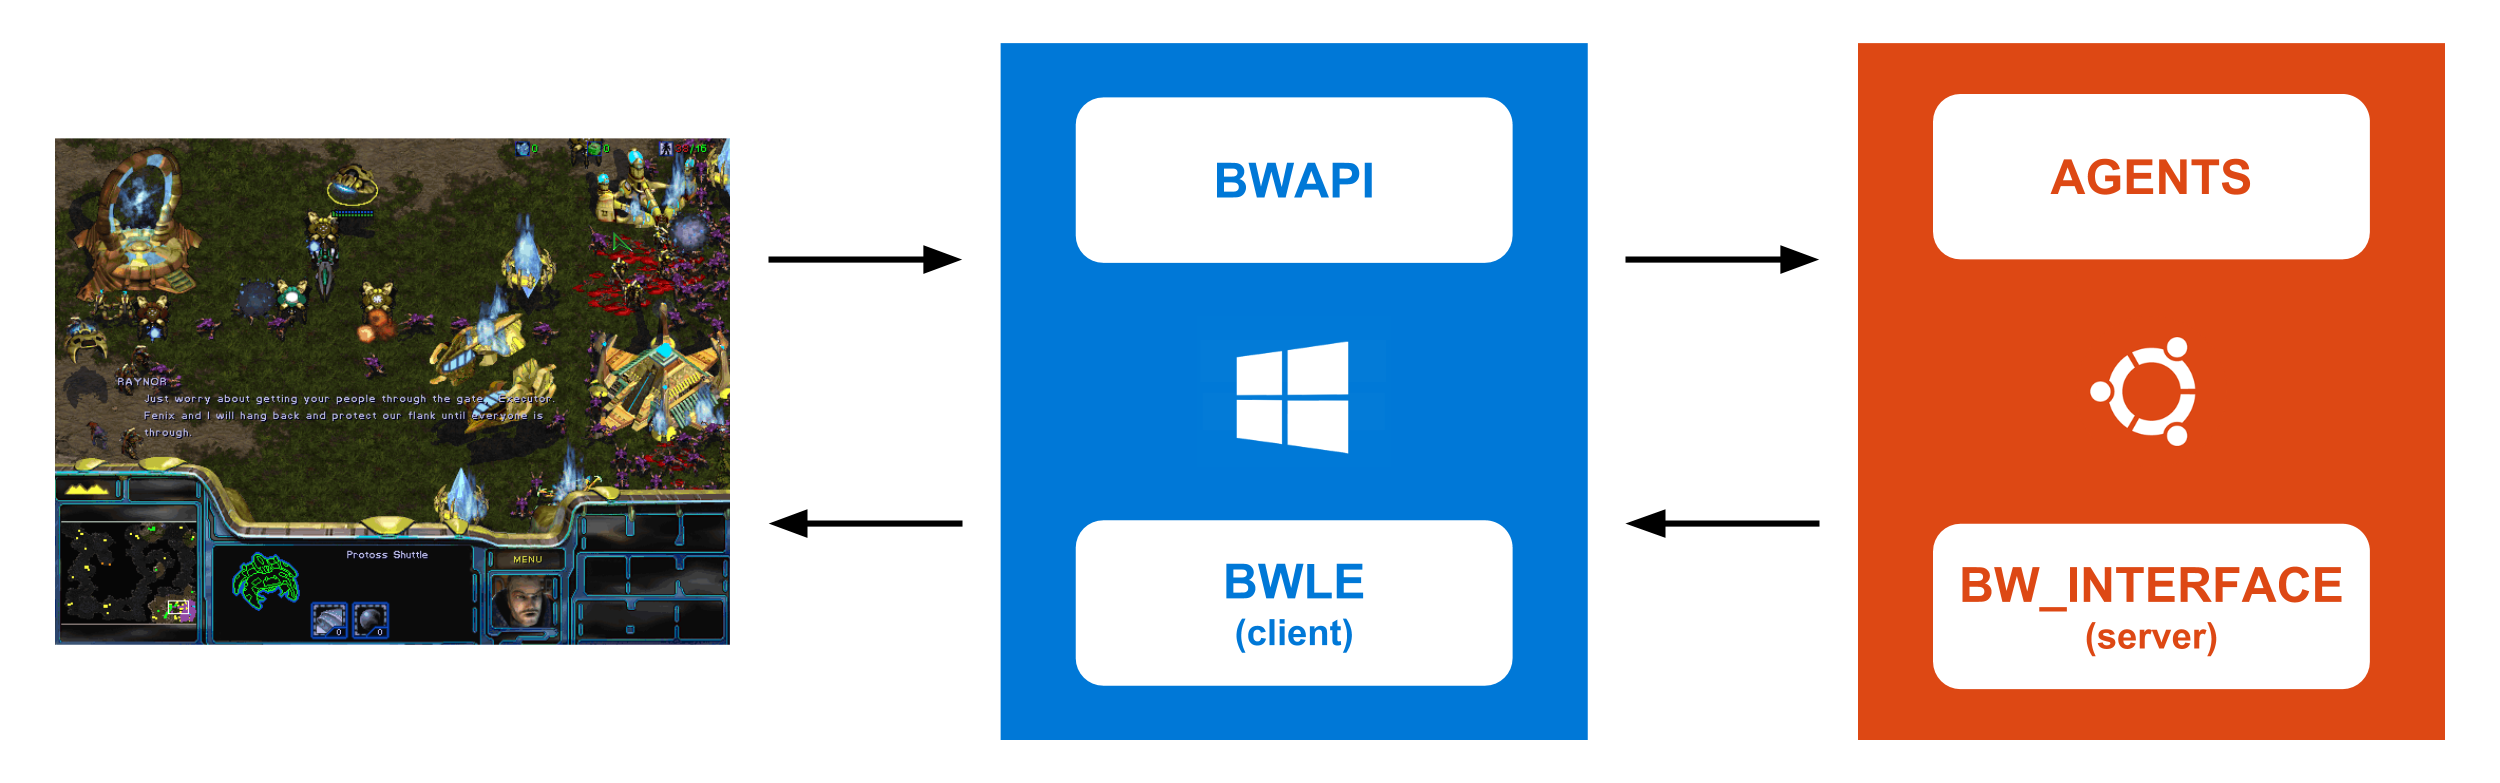
\includegraphics[width=\textwidth]{ch3/arch_overall}
    \caption{Overall architecture. The interface running on Windows 7
      communicates with StarCraft using BWAPI, and connects to a Linux server
      using standard non-blocking sockets. The Linux interfaces communicates
      with an agent through shared objects, }
    \label{fig:arch_ov}
\end{figure}

The two separate systems communicate between each other using non-blocking
sockets in a synchronous or asynchronous fashion depending on how the interface
is configured. The choice is dependent mostly on the experimental design:

\begin{itemize}
\item synchronous communication to simulate the standard MDP-like setting where
  at each step all agents receive the entirety of all observable data, the
  environment is blocked until the decision process has finished and the
  environment executes a step when the MDP processes send a certain command. 
\item asynchronous communication to have a closer simulation to real-world
  scenarios and games. In this mode the game executes each step at a fixed rate
  and sends information as fast as possible (as the game steps rate can be much
  faster than it's currently possible to process and send the visual data). The
  agent can then send actions at any point of the process, which are then
  executed in the next immediate step.
\end{itemize}

To be as efficient and fast as possible, the data structures containing the game
data are serialised using the Google protobuf library \citep{varda2008protocol}.
The library provides a way to generate serialised objects using pre-defined
schemas, which can then be filled with game information and sent over as
compressed strings. Unfortunately the library is not optimised for very large
objects, so we in addition implemented our own serialisation method for
sending the image structure over the socket connection.

While both systems works, the asynchronous interface requires a significant
amount of work on the agent side to sync the data sources and take into account
the perception/action delay. Such processes are generally considered a source of
research problems, but they are not of great interest to decision making, as
once the system is modelled it just becomes part of the environment.

For the sake of clarity and brevity we will from now on describe the rest of the
system only with respect to the synchronous communication, as the implementation
of the rest of the modules is mostly independent from this choice and it greatly
simplifies the agent interface.

\subsection{Windows Interface}

Implemented in C++

Automatically starts the game and injects BWAPI.ddl using ddlinjector. 

\subsubsection{StarCraft Controller}

BWAPI configuration is parsed and edited according to variables specified in the
client configuration system. The idea is to completely hide BWAPI and present a
unique and coherent configuration system with useful defaults.

A list of maps can be load in the system by specifying a file to be parsed. The
game can then be set to load maps sequentially or in random order, which is an
essential feature for standard training procedures.

Games can be interrupted, terminated or restarted at any time. The client allows
to either completely kill StarCraft, therefore resetting its state with a
process-wide restart, or to just use the in-game restart function to quit the
game and start a new one. The first method allows to change certain settings
that can be loaded only when StarCraft is started, but it's significantly
slower, as it takes around two seconds on a quad-core machine from issuing the
kill command and the first step of a new game. The second method takes around a
second to start another game. % CITATION NEEDED (check starcraft times)

% TODO: add seed to game if possible, otherwise future work

% insert example files here 

\subsubsection{Screen capturing}

% TODO describe window size

BWAPI does not provide any interface to capture the visual output of the
game\footnote{Some work had been previously done to integrate some form of
  streaming functionality within BWAPI, but it was dropped in favour of existing
  tools. See https://github.com/bwapi/bwapi/issues/596}. To fulfill the
specifications we developed a module to capture the StarCraft window and include
it in the game state.

\begin{figure}[h]
    \centering
    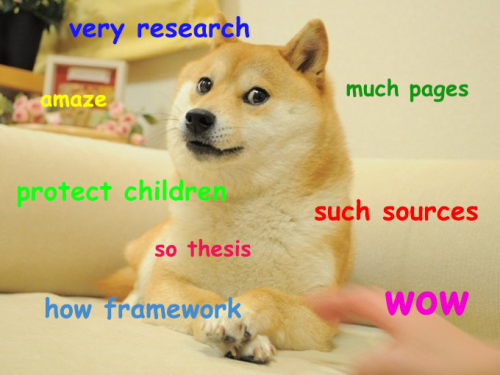
\includegraphics[width=\textwidth]{placeholder}
    \caption{Conversion process of the visual data. The raw pixel data captured
      using the window handler gets stripped of superfluous data and separated
      by channel at the same time.}
    \label{fig:capt_conv}
\end{figure}


To achieve this functionality we used the Graphics Device Interface library
Gdiplus, included as part of the standard Windows API, to find the StarCraft
process, grab its window's handler and extract the raw pixel data. The obtained
data structure stores the pixel in an array of 32bit integers, where integer
represent the row-wise RGB data and a null byte. 

Before serialising the data to use the network endianness order over the wire,
we strip the null byte and we cluster the channels separately as to obtain first
all the red channel values, then the gree channel values, and finally the blue
channel values (Figure \ref{fig:capt_conv}). It must be noted that while this
process has been made as fast as possible on the single thread (given the frame
size), it could be even further optimised by using the fact that the channels
are essentially already independent and therefore using a standard parallel loop
and some pointer map to shift the array around.

% TODO describe image serialisation

\subsubsection{Collecting the Game State}

Collecting the game state represented a non-trivial design and implementation
challenge. BWAPI is designed with in mind the process of writing classical AI
bots, which usually does not include getting access to the entirety of the game
data structures. This means that the interface is modular and divided with
respect to unit classes, weapons, available upgrades, events, forces and so on.
Collecting the game state in a straightforward manner means therefore querying
most of the internal interface, filtering out errors and unneeded information,
and finally clustering everything to fit our shared data structures. 

\begin{algorithm}[H]
\SetAlgoLined
\KwResult{Write here the result }
 initialization\;
 \While{While condition}{
  instructions\;
  \eIf{condition}{
   instructions1\;
   instructions2\;
   }{
   instructions3\;
  }
 }
 \caption{How to write algorithms}
 \label{alg:state}
\end{algorithm}

To do so we developed a module called \texttt{StateManager} to take the burden
of doing all the necessary operations. Algorithm \ref{alg:state} describes the
rough process. Once the state is collected, the module serialises it and sends
it over with the previously collected image. As described in the section
introduction, we use a protobuffer to serialise the game state so that it can be
sent over the wire and parsed by the server running on the Linux end.

\subsubsection{Controlling units}



\subsection{Linux Interface}

\subsubsection{Torch}

\subsubsection{LuaJIT-based Implementation}

\section{Algorithmic Interface}

\subsection{Q-learning}

\subsection{DQN}

\subsubsection{Multi-unit DQN}

\section{Remainin Implementation Details}

\section{Summary}

In this chapter we have outlined the motivations behind different chosen
designs, we have described our implementation, and we have covered the algorithms
used for testing and baseline construction.

Designing, implementing and testing the platform took well over 800 hours, and a
couple of separate hundreds of hours were spent reproducing different
implementations of Q-learning and Deep Q-networks. Unfortunately a lot of time
was spent refactoring and dealing with the complex behaviour of Windows APIs and
StarCraft, but the obtained interface seems more than satisfactory.
